%
% ---------------------------------------------------------------
% Copyright (C) 2012-2018 Gang Li
% ---------------------------------------------------------------
%
% This work is the default powerdot-tuliplab style test file and may be
% distributed and/or modified under the conditions of the LaTeX Project Public
% License, either version 1.3 of this license or (at your option) any later
% version. The latest version of this license is in
% http://www.latex-project.org/lppl.txt and version 1.3 or later is part of all
% distributions of LaTeX version 2003/12/01 or later.
%
% This work has the LPPL maintenance status "maintained".
%
% This Current Maintainer of this work is Gang Li.
%
%

\documentclass[
 size=14pt,
 paper=smartboard,  %a4paper, smartboard, screen
 mode=present, 		%present, handout, print
 display=slides, 	% slidesnotes, notes, slides
 style=tuliplab,  	% TULIP Lab style
 pauseslide,
 fleqn,leqno]{powerdot}


\usepackage{cancel}
\usepackage{caption}
\usepackage{stackengine}
\usepackage{smartdiagram}
\usepackage{attrib}
\usepackage{amssymb}
\usepackage{amsmath} 
\usepackage{amsthm} 
\usepackage{mathtools}
\usepackage{rotating}
\usepackage{graphicx}
\usepackage{boxedminipage}
\usepackage{rotate}
\usepackage{calc}
\usepackage[absolute]{textpos}
\usepackage{psfrag,overpic}
\usepackage{fouriernc}
\usepackage{pstricks,pst-3d,pst-grad,pstricks-add,pst-text,pst-node,pst-tree}
\usepackage{moreverb,epsfig,subfigure}
\usepackage{color}
\usepackage{booktabs}
\usepackage{etex}
\usepackage{breqn}
\usepackage{multirow}
\usepackage{natbib}
\usepackage{bibentry}
\usepackage{gitinfo2}
\usepackage{siunitx}
\usepackage{nicefrac}
%\usepackage{geometry}
%\geometry{verbose,letterpaper}
\usepackage{media9}
\usepackage{animate}
%\usepackage{movie15}
\usepackage{auto-pst-pdf}

\usepackage{breakurl}
\usepackage{fontawesome}
\usepackage{xcolor}
\usepackage{multicol}



\usepackage{verbatim}
\usepackage[utf8]{inputenc}
\usepackage{dtk-logos}
\usepackage{tikz}
\usepackage{adigraph}
%\usepackage{tkz-graph}
\usepackage{hyperref}
%\usepackage{ulem}
\usepackage{pgfplots}
\usepackage{verbatim}
\usepackage{fontawesome}


\usepackage{todonotes}
% \usepackage{pst-rel-points}
\usepackage{animate}
\usepackage{fontawesome}

\usepackage{listings}
\lstset{frameround=fttt,
frame=trBL,
stringstyle=\ttfamily,
backgroundcolor=\color{yellow!20},
basicstyle=\footnotesize\ttfamily}
\lstnewenvironment{code}{
\lstset{frame=single,escapeinside=`',
backgroundcolor=\color{yellow!20},
basicstyle=\footnotesize\ttfamily}
}{}


\usepackage{hyperref}
\hypersetup{ % TODO: PDF meta Data
  pdftitle={Presentation Title},
  pdfauthor={Gang Li},
  pdfpagemode={FullScreen},
  pdfborder={0 0 0}
}


% \usepackage{auto-pst-pdf}
% package to show source code

\definecolor{LightGray}{rgb}{0.9,0.9,0.9}
\newlength{\pixel}\setlength\pixel{0.000714285714\slidewidth}
\setlength{\TPHorizModule}{\slidewidth}
\setlength{\TPVertModule}{\slideheight}
\newcommand\highlight[1]{\fbox{#1}}
\newcommand\icite[1]{{\footnotesize [#1]}}

\newcommand\twotonebox[2]{\fcolorbox{pdcolor2}{pdcolor2}
{#1\vphantom{#2}}\fcolorbox{pdcolor2}{white}{#2\vphantom{#1}}}
\newcommand\twotoneboxo[2]{\fcolorbox{pdcolor2}{pdcolor2}
{#1}\fcolorbox{pdcolor2}{white}{#2}}
\newcommand\vpspace[1]{\vphantom{\vspace{#1}}}
\newcommand\hpspace[1]{\hphantom{\hspace{#1}}}
\newcommand\COMMENT[1]{}

\newcommand\placepos[3]{\hbox to\z@{\kern#1
        \raisebox{-#2}[\z@][\z@]{#3}\hss}\ignorespaces}

\renewcommand{\baselinestretch}{1.2}


\newcommand{\draftnote}[3]{
	\todo[author=#2,color=#1!30,size=\footnotesize]{\textsf{#3}}	}
% TODO: add yourself here:
%
\newcommand{\gangli}[1]{\draftnote{blue}{GLi:}{#1}}
\newcommand{\shaoni}[1]{\draftnote{green}{sn:}{#1}}
\newcommand{\gliMarker}
	{\todo[author=GLi,size=\tiny,inline,color=blue!40]
	{Gang Li has worked up to here.}}
\newcommand{\snMarker}
	{\todo[author=Sn,size=\tiny,inline,color=green!40]
	{Shaoni has worked up to here.}}

%%%%%%%%%%%%%%%%%%%%%%%%%%%%%%%%%%%%%%%%%%%%%%%%%%%%%%%%%%%%%%%%%%%%%%%%
% title
% TODO: Customize to your Own Title, Name, Address
%
\title{Bike Sharing Demand
\\Forecast use of a city bikeshare system}
\author{
Dong Zhu
\\
\\ 
\\Deakin University
\\
}
\date{\gitCommitterDate}


% Customize the setting of slides
\pdsetup{
% TODO: Customize the left footer, and right footer
rf=\href{http://www.tulip.org.au}{
Last Changed by: \textsc{\gitCommitterName}\ \gitVtagn-\gitAbbrevHash\ (\gitAuthorDate)
},
cf={Bike Sharing Demand Prediction},
}


\begin{document}

\maketitle

%\begin{slide}{Overview}
%\tableofcontents[content=sections]
%\end{slide}


%%==========================================================================================
%%
\begin{slide}[toc=,bm=]{Overview}
\tableofcontents[content=currentsection,type=1]
\end{slide}
%%
%%==========================================================================================

\section{Problem Definition}


%%==========================================================================================
%%
\begin{slide}{Bike Sharing Demand Prediction}
\begin{center}
\twotonebox{\rotatebox{90}{Definition}}{\parbox{.86\textwidth}
{Bike-sharing systems are a means of renting bikes, through which people can rent a bike from any place and return it when they arrive at their destination.
The bike-sharing system clearly records the time of travel, the place of departure, the place of arrival and the time.
Therefore, it can be used to study mobility in cities.
In this project, historical usage patterns were combined with weather data to predict bike rental demand in Washington, D.C.
\begin{itemize}
\item Researchers can use bike sharing systems  as a sensor network, which can be used for studying mobility in a city.
\item This is a Supervised regression machine learning task.
\item The training set is comprised of the first 19 days of each month, while the test set is the 20th to the end of the month.
\end{itemize}
}}

\end{center}
\end{slide}
%%
%%==========================================================================================

%%==========================================================================================
%%

\section{Data exploration}



%%==========================================================================================
%%
\begin{slide}{Check for missing vaules }



\twocolumn
{
\vspace{0.75cm}
%\vspace{0.1cm}
\begin{figure}
  \centering
  \selectcolormodel{rgb}
  %\missingfigure{Testing a long text string.}
  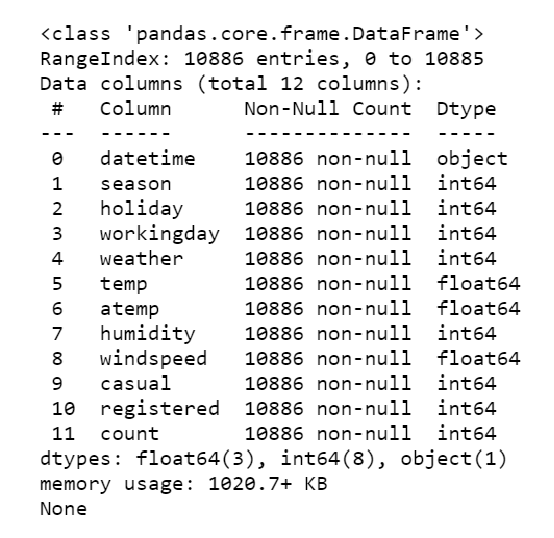
\includegraphics[width=0.6\textwidth]{figures//train_info.eps}\\
  \caption{Training data information}\label{fig:GroupOutAspect-target}
\end{figure}
}
{



\bigskip
\bigskip

\begin{figure}
  \centering
  \selectcolormodel{rgb}
  %\missingfigure{Testing a long text string.}
  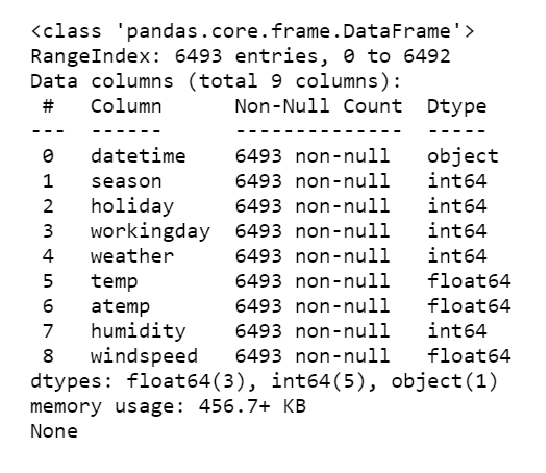
\includegraphics[width=0.6\textwidth]{figures//test_info.eps}\\
  \bigskip
  \caption{Test data information}\label{fig:OutAspect-target}
\end{figure}
}


\end{slide}
%%
%%==========================================================================================


%%==========================================================================================
%%
\begin{slide}{Check for outliers}

\begin{itemize}
\item
Statistical description
\end{itemize}

\begin{figure}
  \centering
  \selectcolormodel{rgb}
  %\missingfigure{Testing a long text string.}
  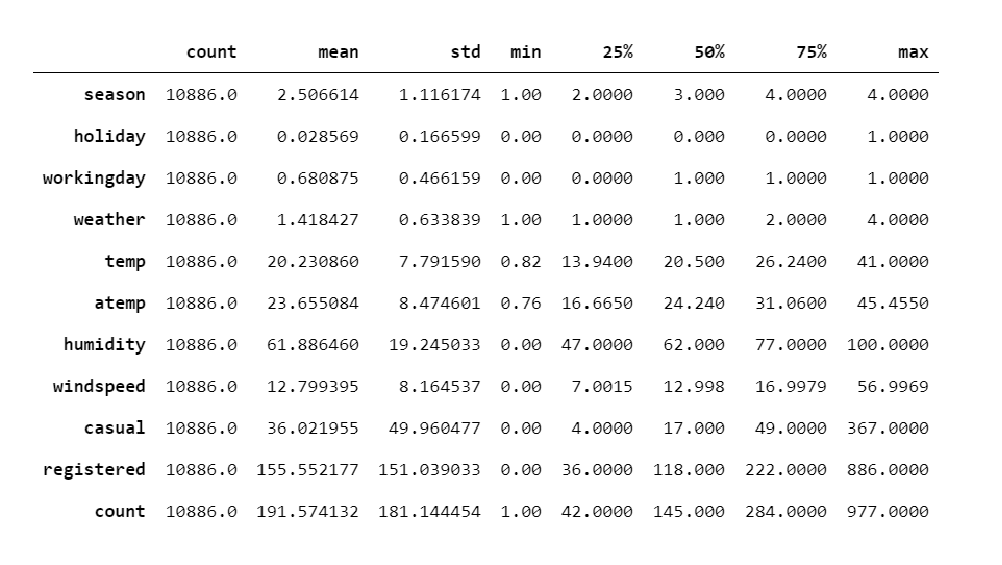
\includegraphics[width=0.6\textwidth]{figures//description.eps}\\
  \bigskip
  \caption{Data description}\label{fig:OutAspect-target}
\end{figure}


\end{slide}
%%
%%==========================================================================================


%%==========================================================================================
%%
\begin{slide}[toc=,bm=]{Check for outliers}


\begin{figure}
  \centering
  \selectcolormodel{rgb}
  %\missingfigure{Testing a long text string.}
  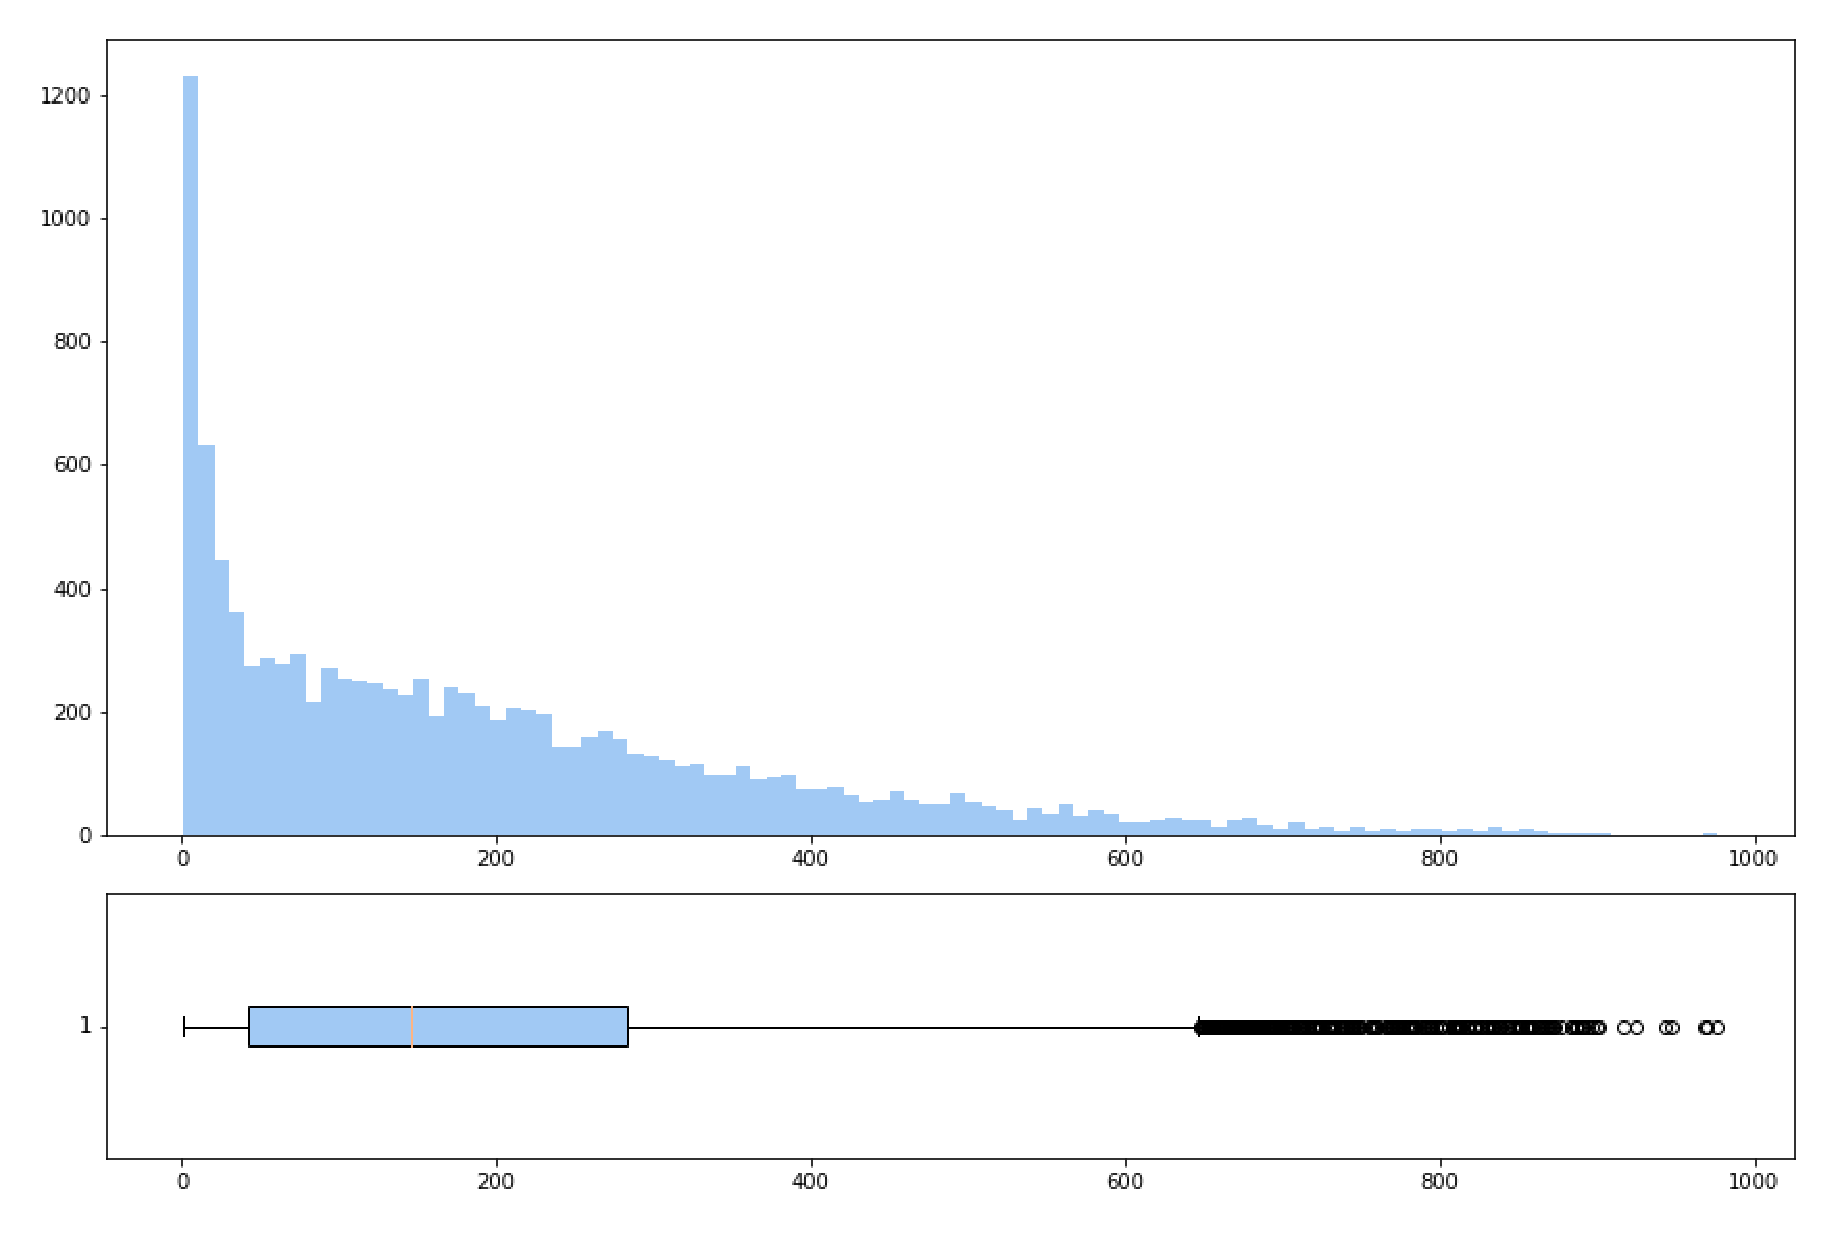
\includegraphics[width=0.6\textwidth]{figures//Count_distribution.eps}\\
  \caption{The distribution of the label "count"}\label{fig:OutAspect-target}
\end{figure}


\end{slide}
%%
%%==========================================================================================


%%==========================================================================================
%%
\begin{slide}[toc=,bm=]{Check for outliers}


\begin{figure}
  \centering
  \selectcolormodel{rgb}
  %\missingfigure{Testing a long text string.}
  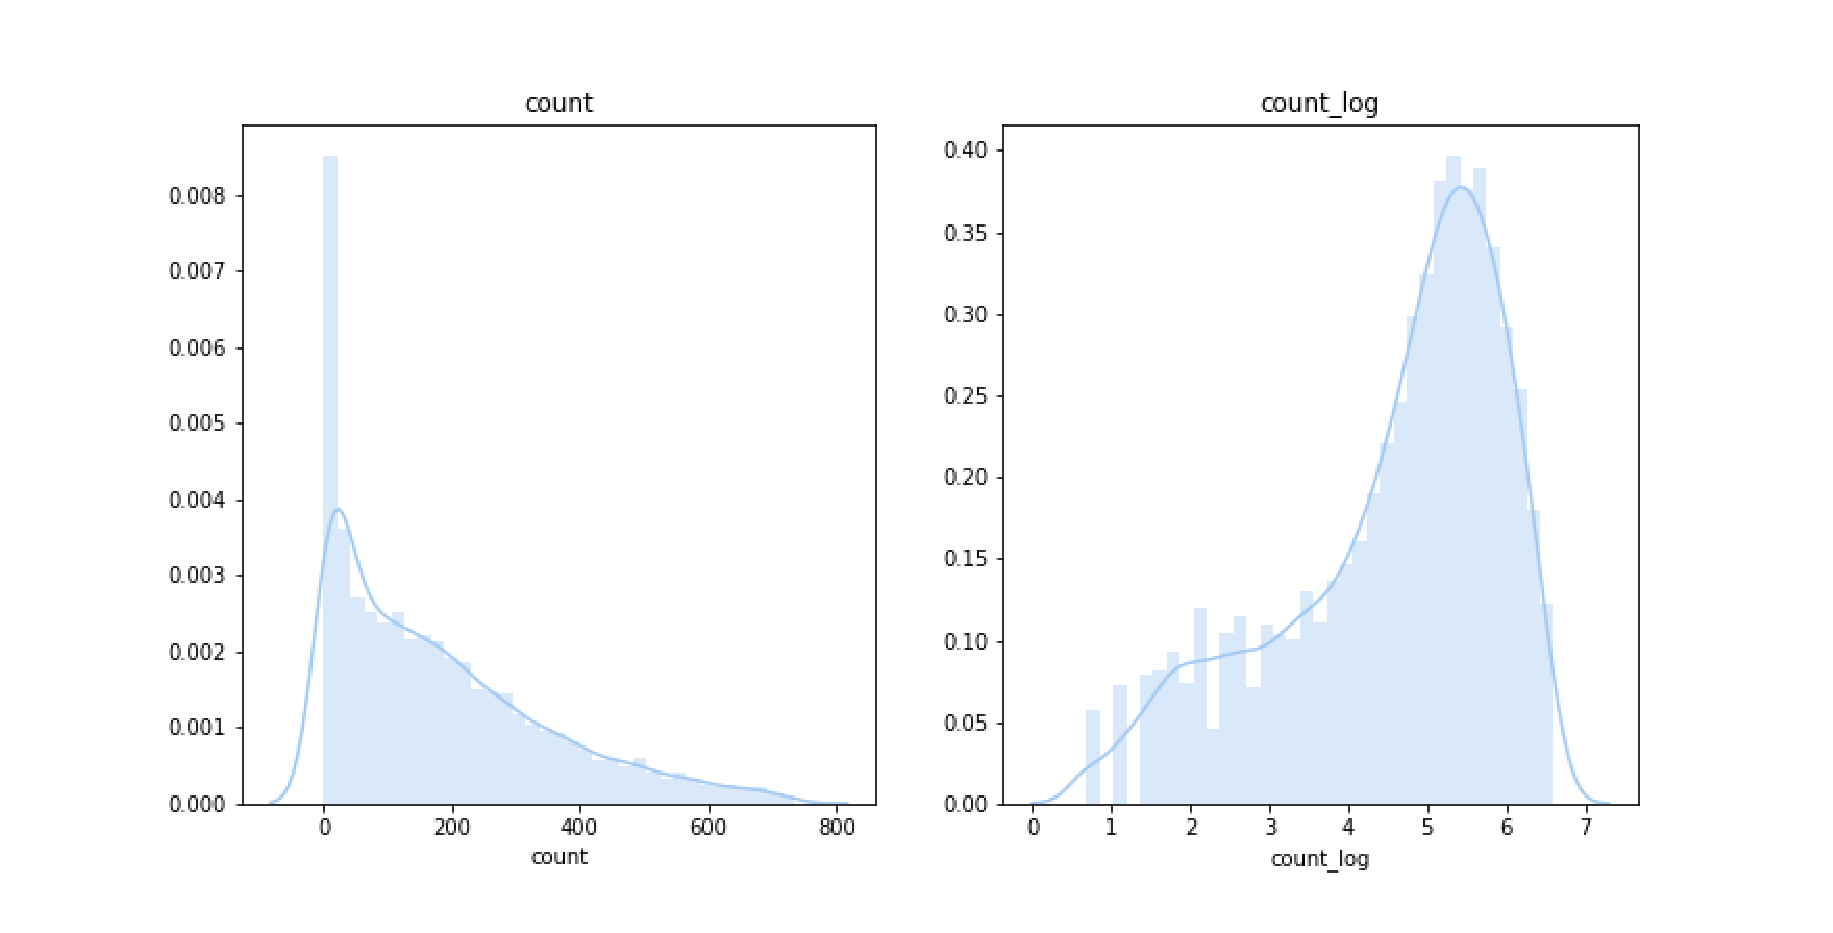
\includegraphics[width=1\textwidth]{figures//Count_distribution_compare.eps}\\
  \caption{Count distribution compare}\label{fig:OutAspect-target}
\end{figure}
  
  


\end{slide}
%%
%%==========================================================================================
%%==========================================================================================
%%
\begin{slide}[toc=,bm=]{Check for outliers}
\vspace{-0.8cm}
\begin{figure}
\centering
\selectcolormodel{rgb}
%\missingfigure{Testing a long text string.}
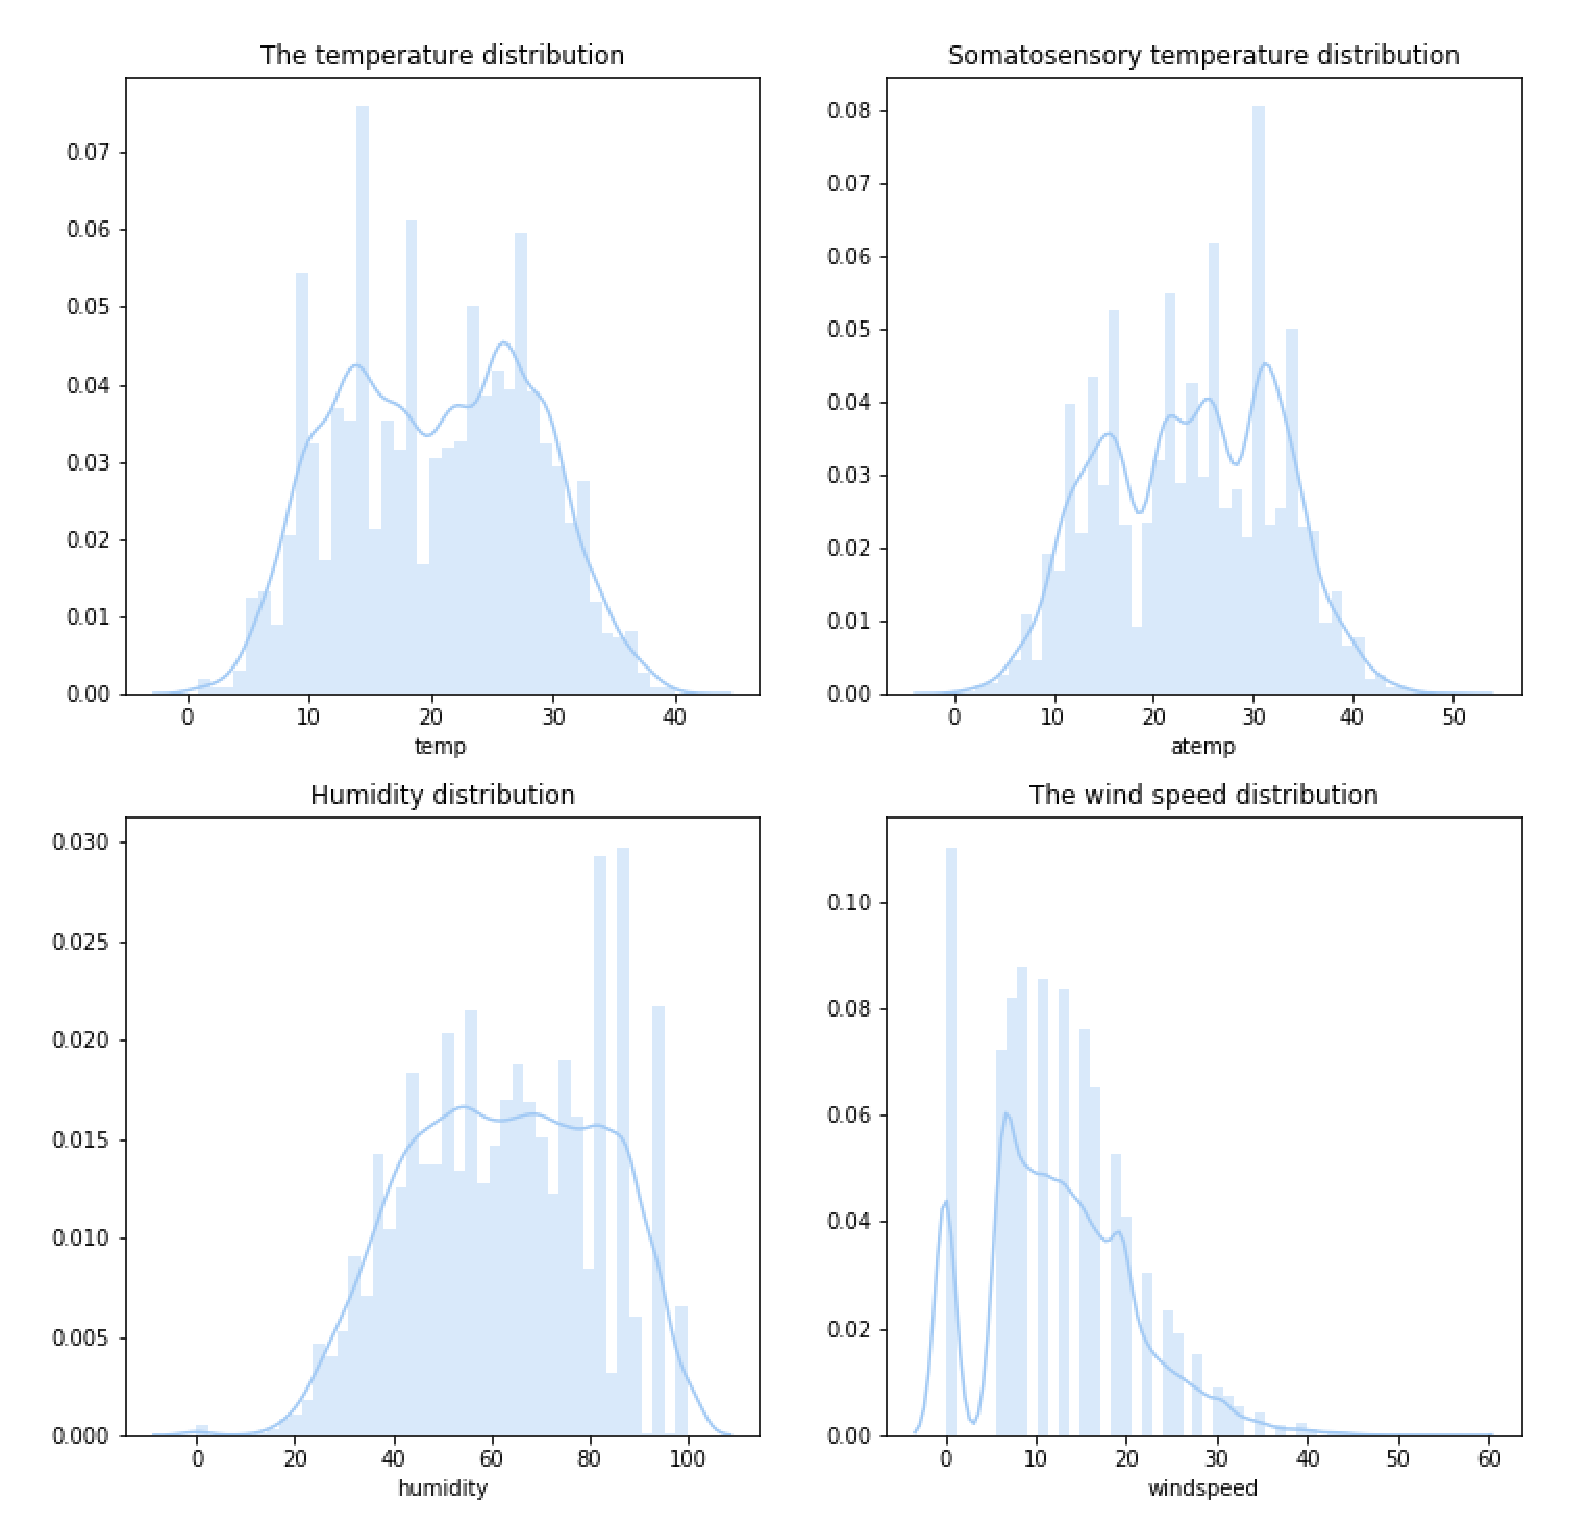
\includegraphics[width=0.6\textwidth]{figures//Features_distribution_analysis.eps}\\
\caption{Main features distribution}\label{fig:OutAspect-target}
\end{figure}
      
\end{slide}
%%
%%==========================================================================================
  
%%==========================================================================================
%%
\begin{slide}[toc=,bm=]{Check for outliers}

 
  
\vspace{-0.8cm}
\begin{figure}
\centering
\selectcolormodel{rgb}
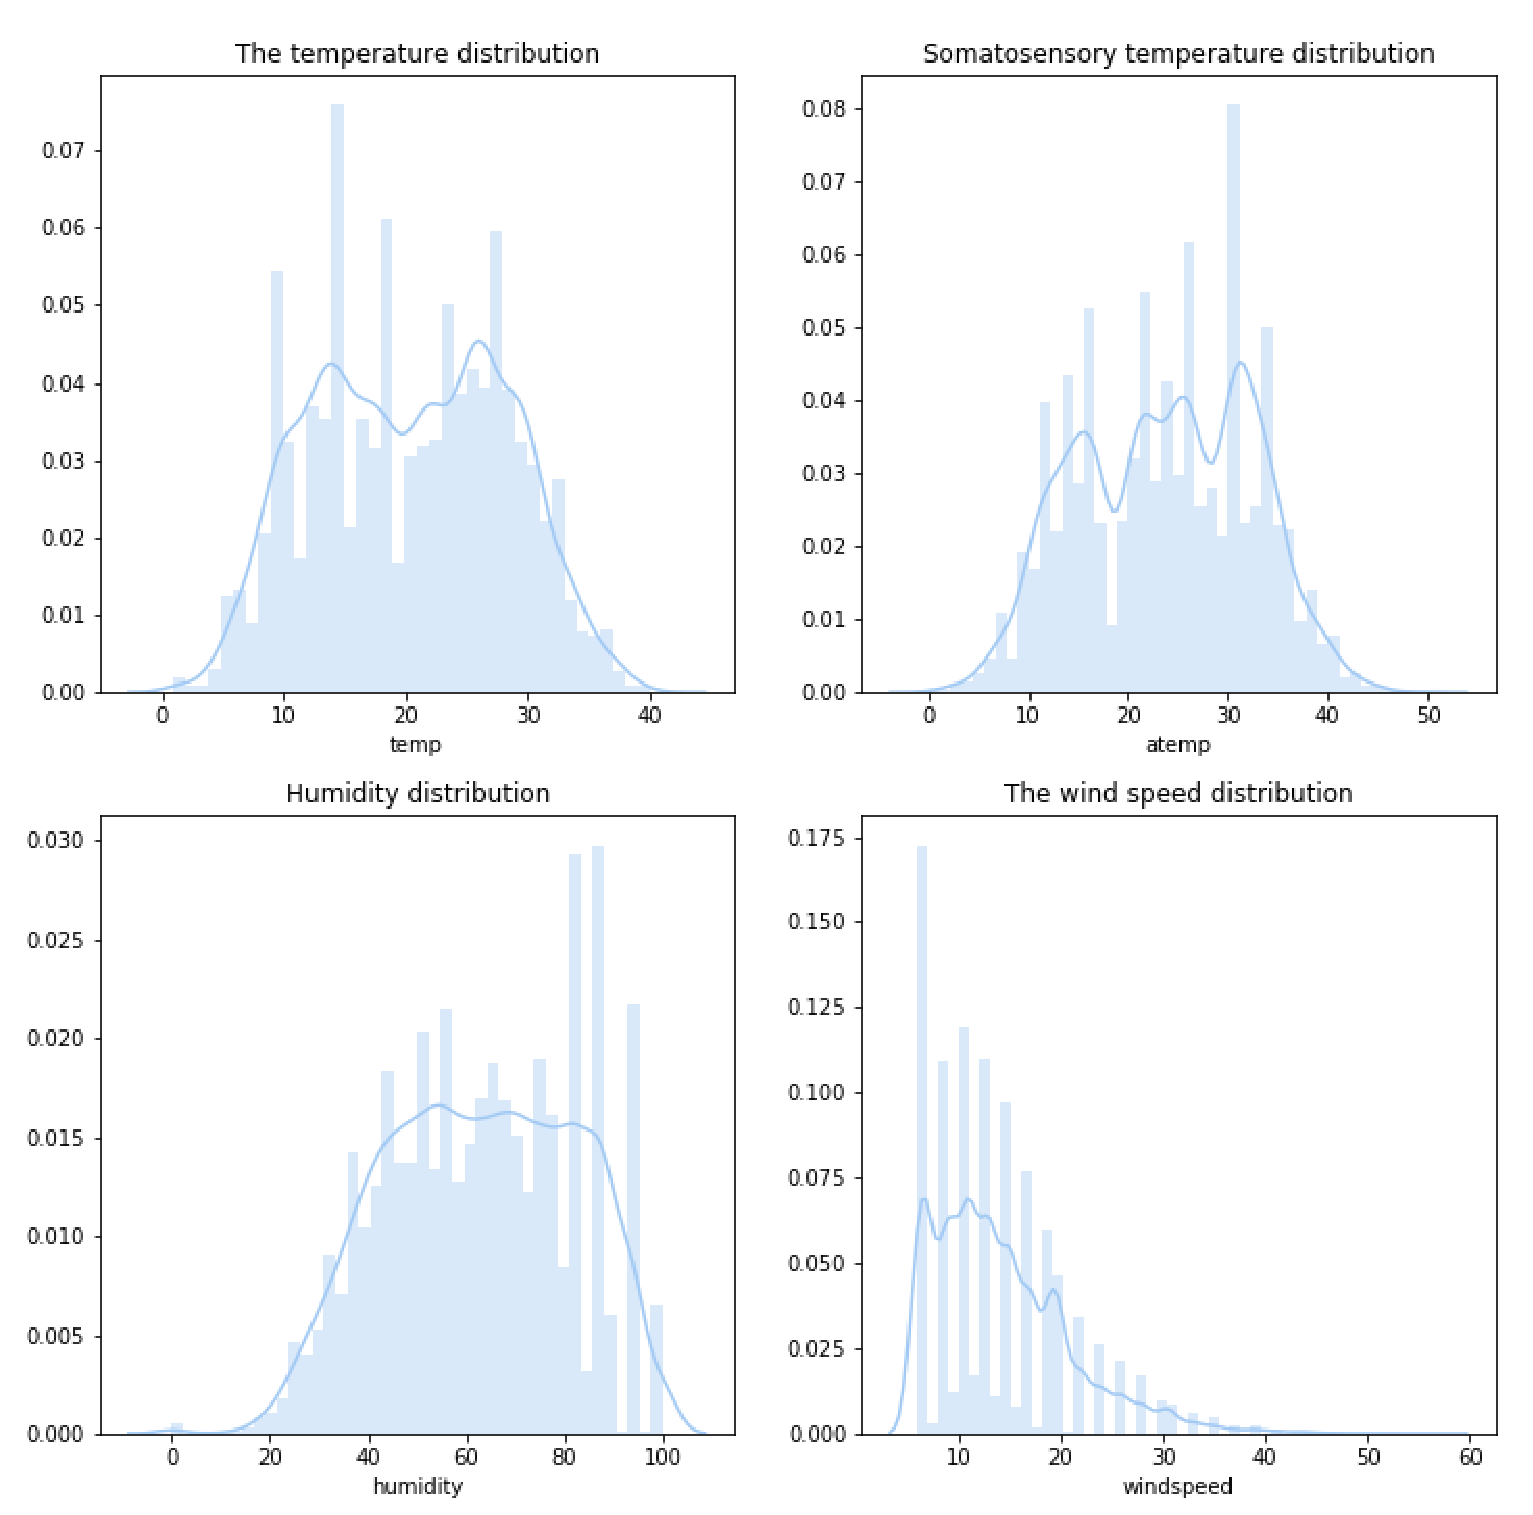
\includegraphics[width=0.5\textwidth]{figures//After_features_distribution_analysis.eps}\\
\caption{Main features distribution}\label{fig:OutAspect-target}
\end{figure}
        
\end{slide}
%%
%%==========================================================================================
   
\section{Data visualization}


%%==========================================================================================
%%
\begin{slide}{Time characteristic analysis}

\begin{itemize}
\item
there are two peaks in the graph, one is from 7-8 in the morning, 
the other is from 5-6 in the afternoon, which is the morning peak 
and the evening peak respectively, which is in line with the actual situation. 
\end{itemize} 
\vspace{-0.8cm} 
\begin{figure}
  \centering
  \selectcolormodel{rgb}
%  \missingfigure{Testing a long text string.}
  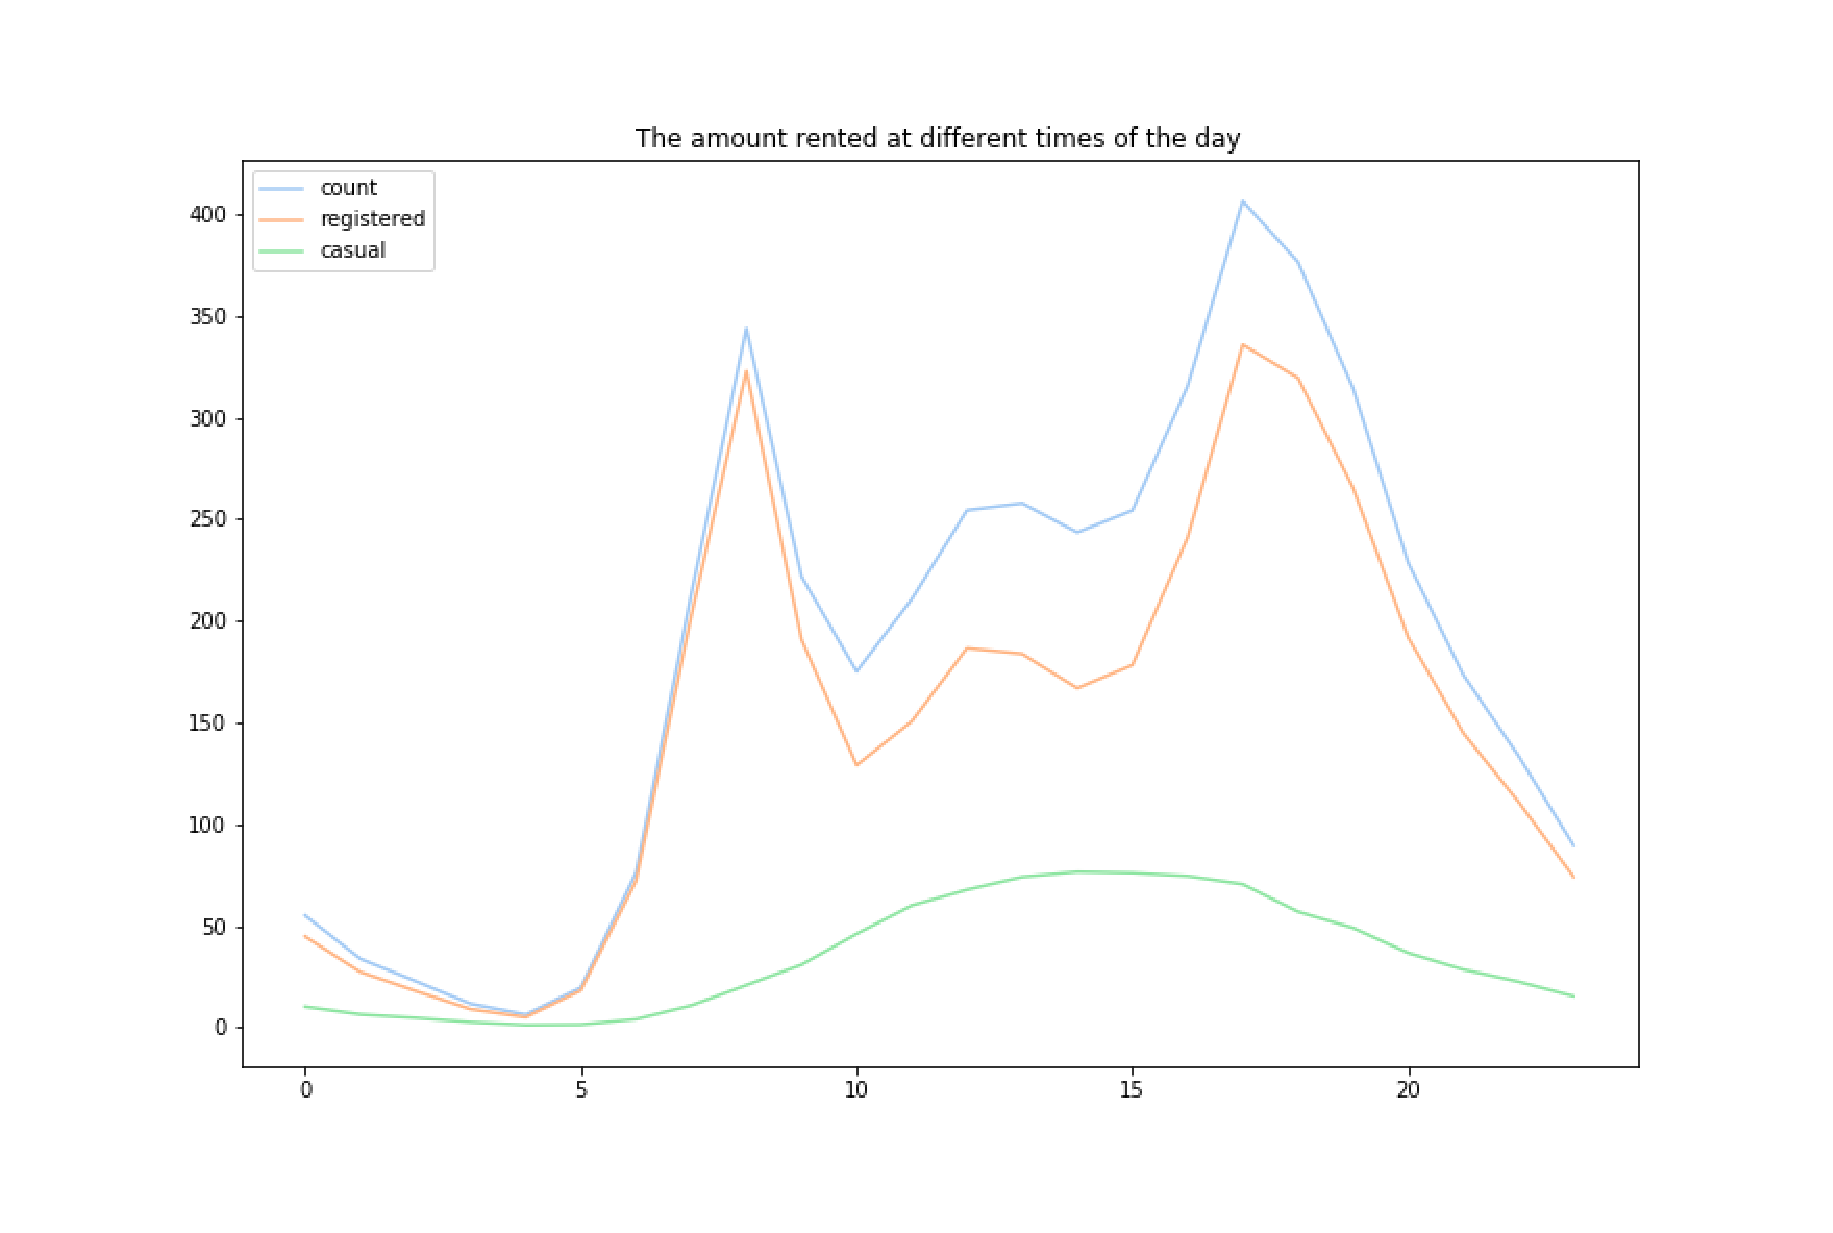
\includegraphics[width=0.6\textwidth]{figures//Time_trends_day.eps}\\
  \caption{The amount rented at different times of the day} \label{framework}
\end{figure}


\end{slide}
%%
%%==========================================================================================

%%==========================================================================================
%%
\begin{slide}[toc=,bm=]{Time characteristic analysis}

\begin{itemize}
\item
from Monday to Friday, 8 in the morning of the day - 9 am and 5 to 7 PM, 
usage is more, may be caused by time going to work in the morning and 
evening after work time, include the reason of eating out at the same time,
 for the weekend, time is more focused, basic usage around 11 PM to 5 PM, 
 This time is supposed to be everyone's leisure time.
\end{itemize} 
\vspace{-1cm}  
\begin{figure}
  \centering
  \selectcolormodel{rgb}
%  \missingfigure{Testing a long text string.}
  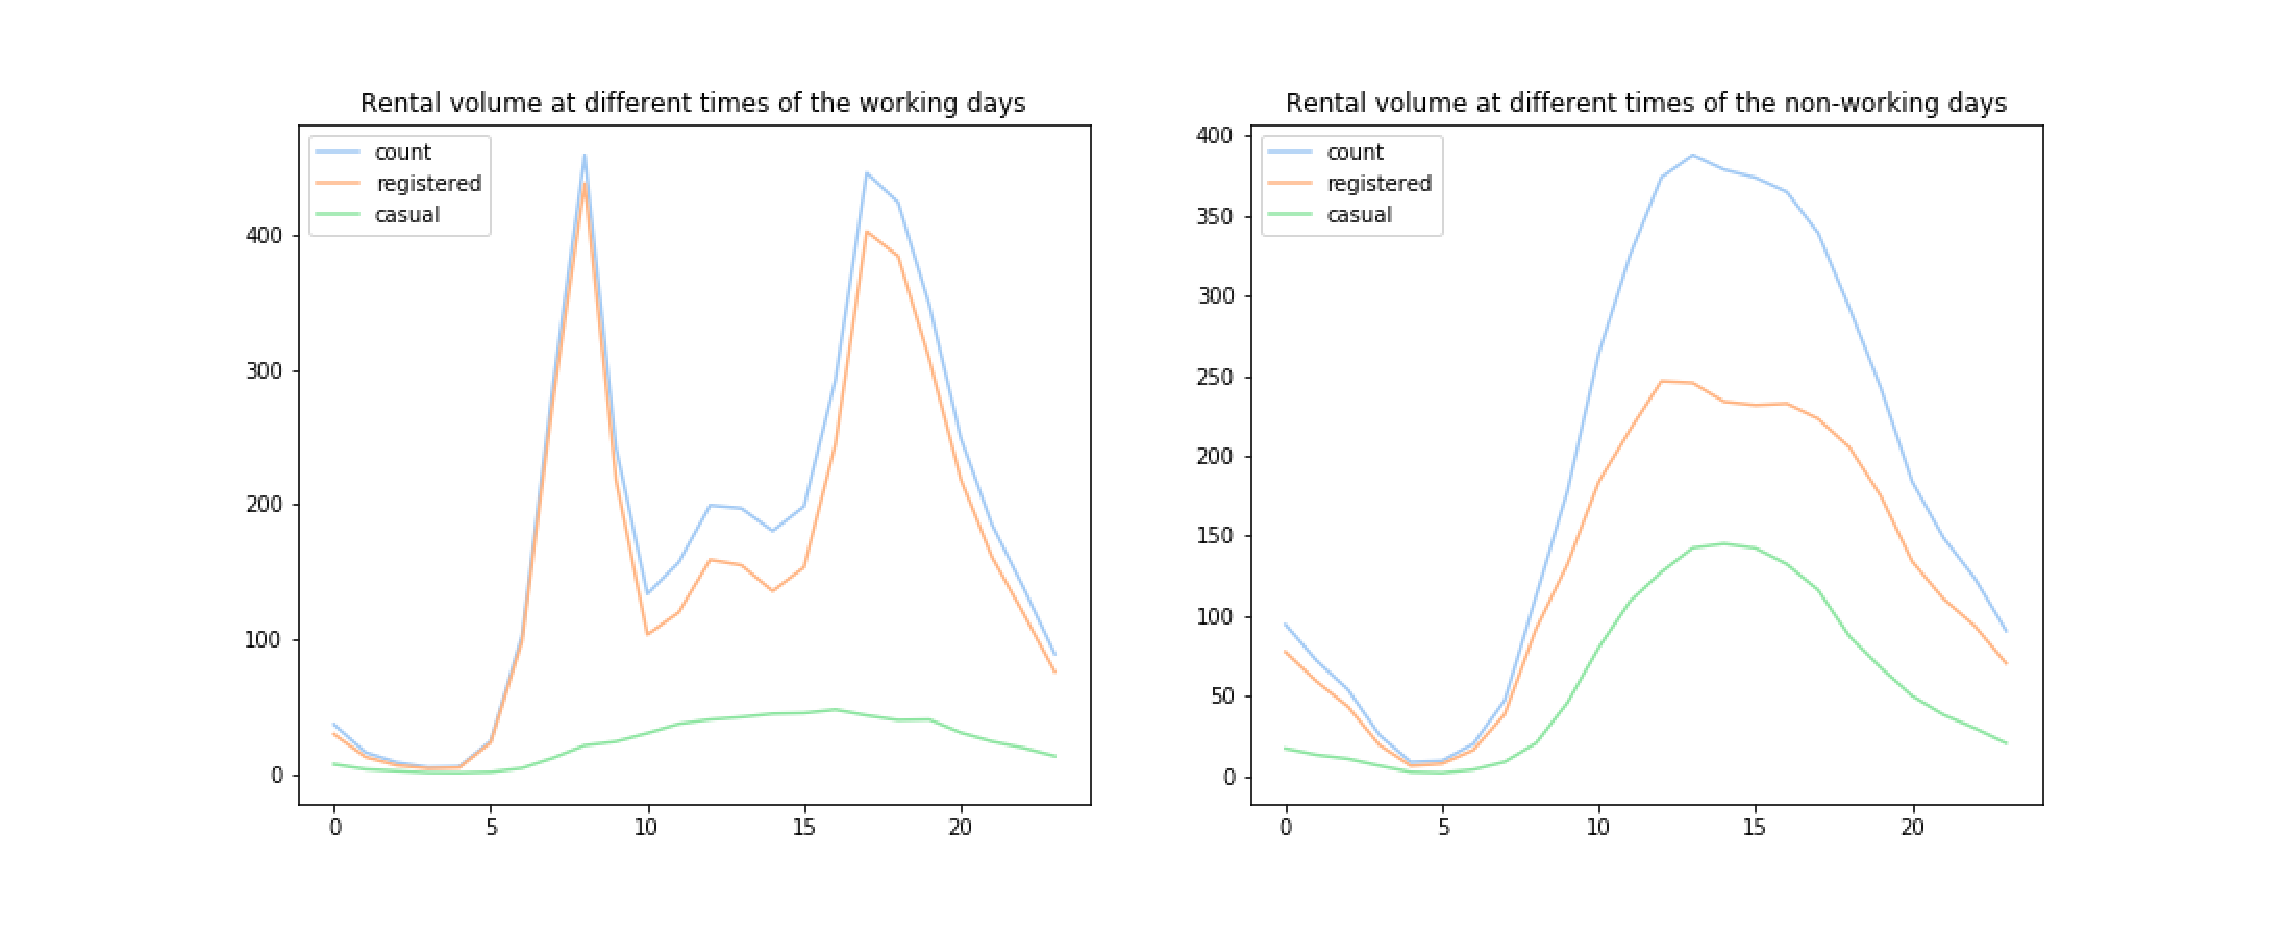
\includegraphics[width=0.7\textwidth]{figures//time_trends_weekday.eps}\\
  \caption{Rental amount at different times of the non-working days and the non-working days} \label{framework}
\end{figure}
  
  
\end{slide}
%%
%%==========================================================================================

%%==========================================================================================
%%
\begin{slide}[toc=,bm=]{Time characteristic analysis}

\begin{itemize}
\item
The usage is obviously lower in spring,
probably due to the lower temperature. 
\end{itemize} 
    
\begin{figure}
  \centering
  \selectcolormodel{rgb}
  %  \missingfigure{Testing a long text string.}
  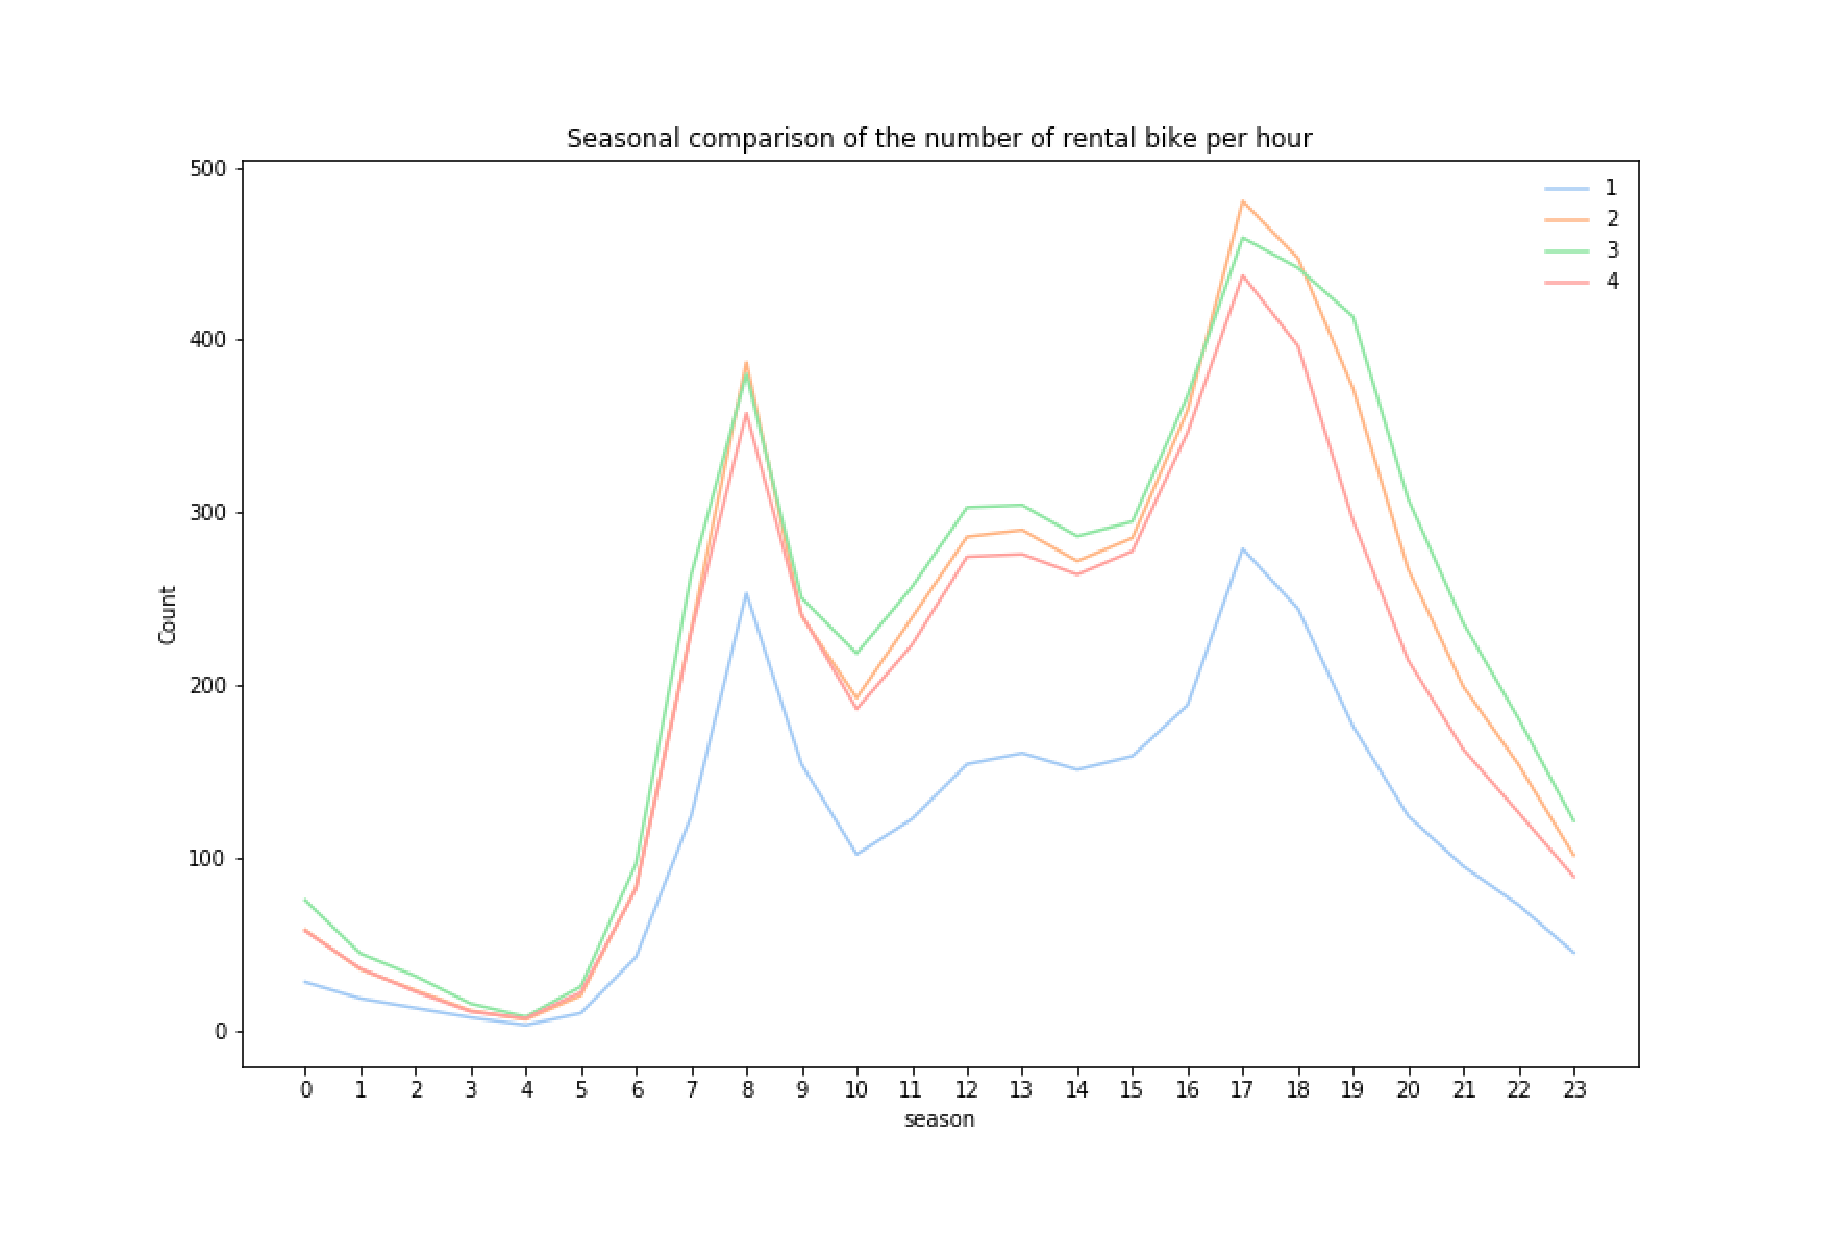
\includegraphics[width=0.6\textwidth]{figures//season.eps}\\
  \caption{Seasonal comparison of the number of rental bike per hour} \label{framework}
\end{figure}
    
    
\end{slide}
%%
%%==========================================================================================

%%==========================================================================================
%%
\begin{slide}{Weather characteristics analysis}
  \begin{itemize}
    \item
    Temperatures below 10 degrees, above 30 degrees, and fewer bike rentals -- too cold or too hot will damper rental demand. 
    \item
    The higher the wind, the fewer bike renters - high winds dampen rental demand.
    \item
    The higher the humidity in the air, the fewer people who hire bikes - it's more comfortable to ride on dry days.
    \end{itemize}
  \vspace{-1.5cm}
  \begin{figure}
    \centering
    \selectcolormodel{rgb}
    %  \missingfigure{Testing a long text string.}
    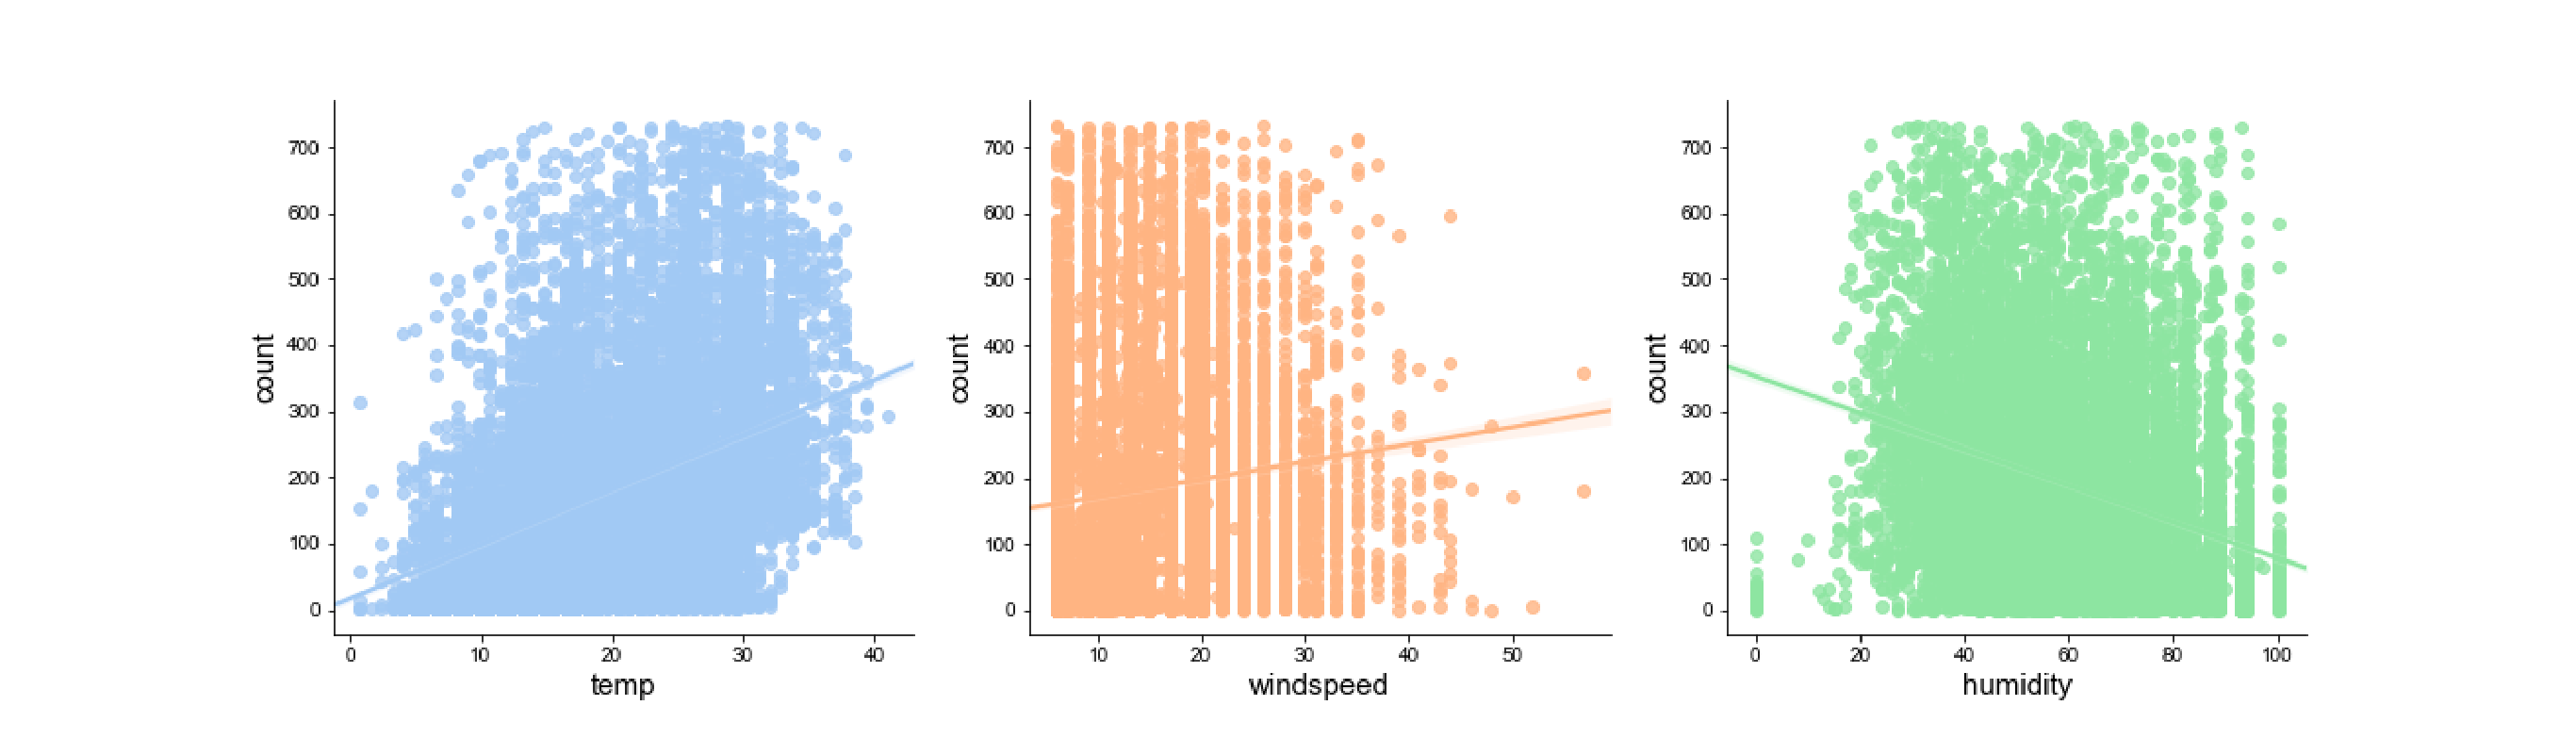
\includegraphics[width=1\textwidth]{figures//weather.eps}\\
    \caption{The effect of weather on rental amount} \label{framework}
  \end{figure}
      
      
  \end{slide}
%%
%%==========================================================================================
\section{Feature selection}


%%==========================================================================================
%%
\begin{slide}{Correlation analysis}
  \vspace{-1cm}
  \begin{figure}
  \centering
  \selectcolormodel{rgb}
%  \missingfigure{Testing a long text string.}
  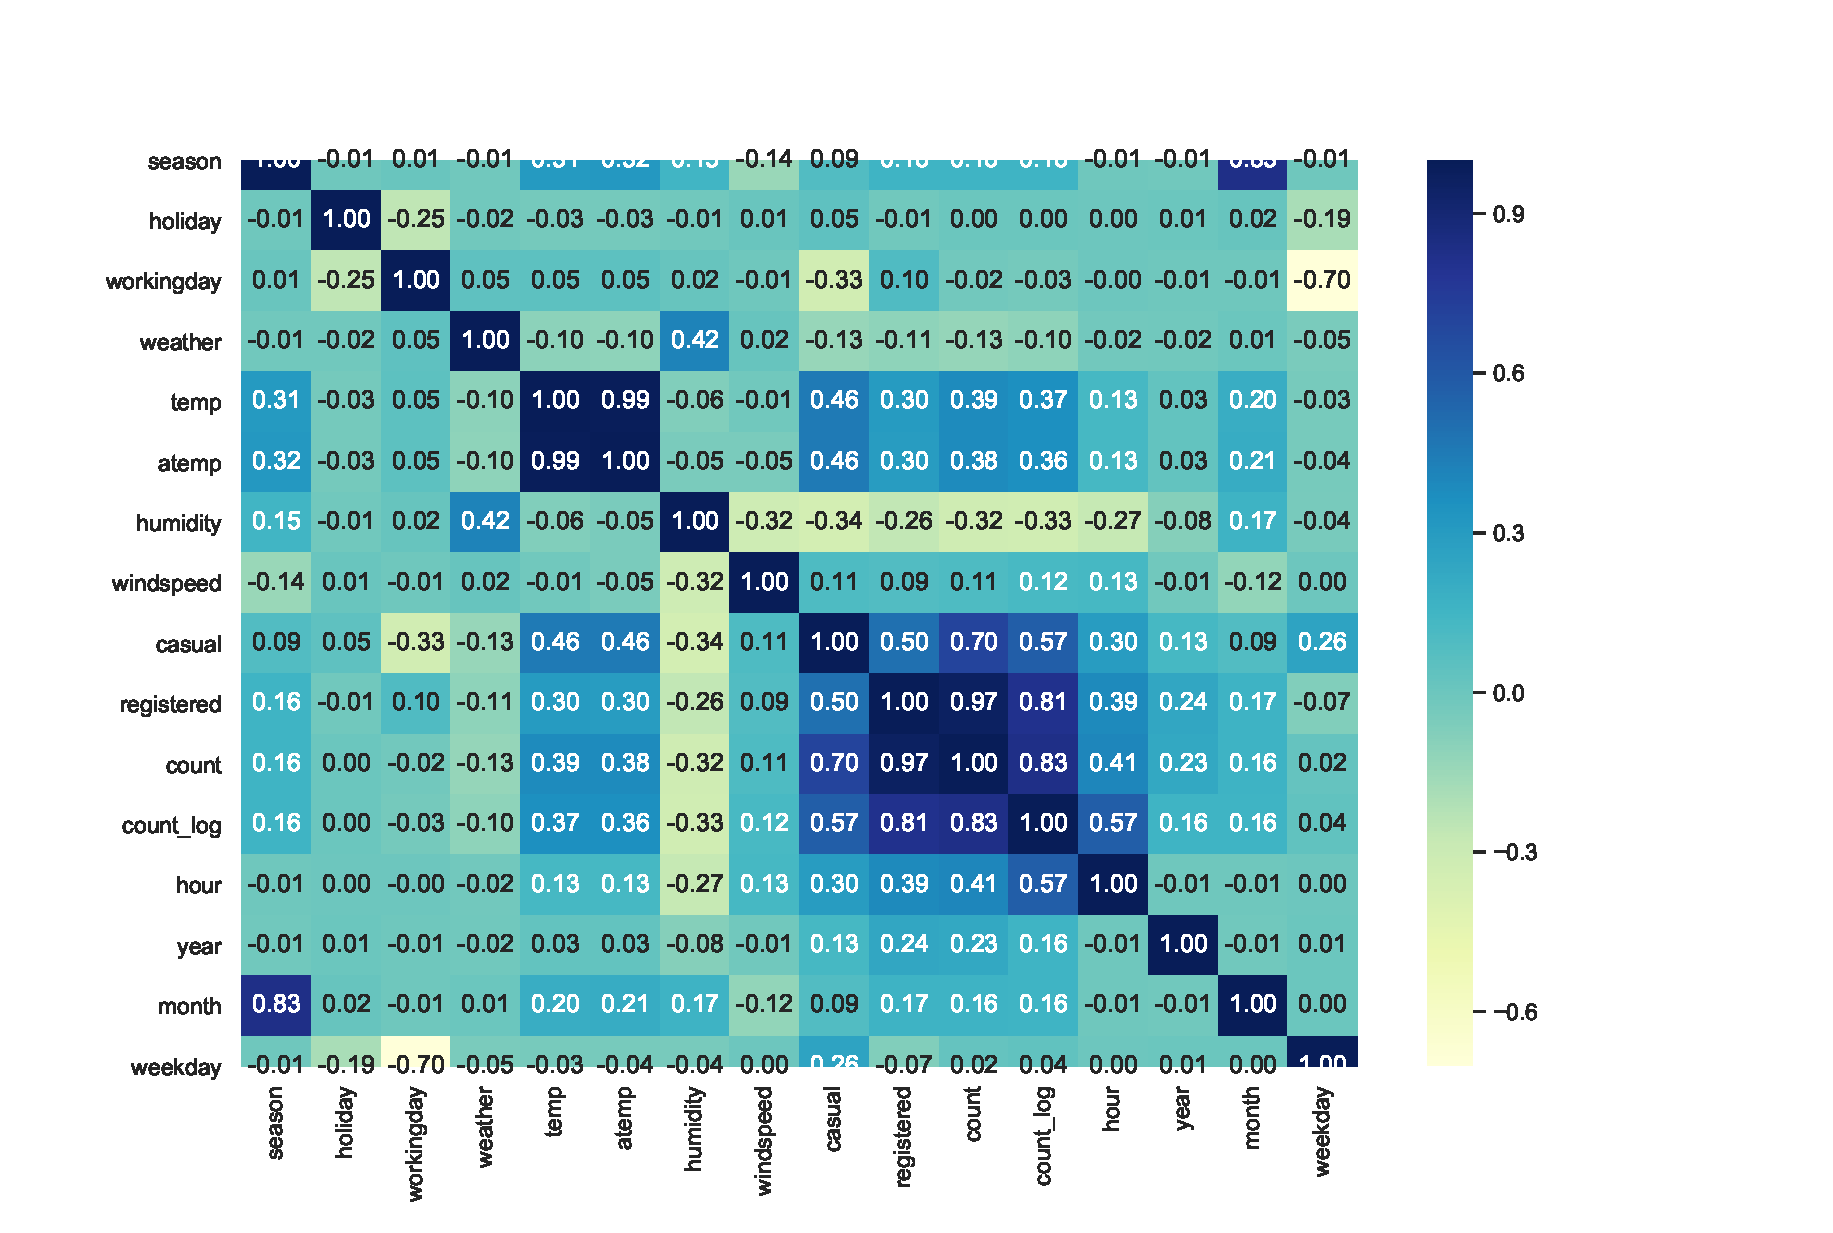
\includegraphics[width=0.8\textwidth]{figures//cor.eps}\\
  \caption{Correlation analysis} \label{framework}
\end{figure}


\end{slide}
%%
%%==========================================================================================
%%==========================================================================================
%%
\begin{slide}[toc=,bm=]{Correlation analysis}
  \begin{itemize}
    \item
    The influence of characteristics on count is as follows: 
    hour>temp>atemp>humidity>month>season>year>weather>windspeed
    >workingday>weekday>day>holiday
    \end{itemize}
  \vspace{-0.8cm}
  \begin{figure}
    \centering
    \selectcolormodel{rgb}
  %  \missingfigure{Testing a long text string.}
    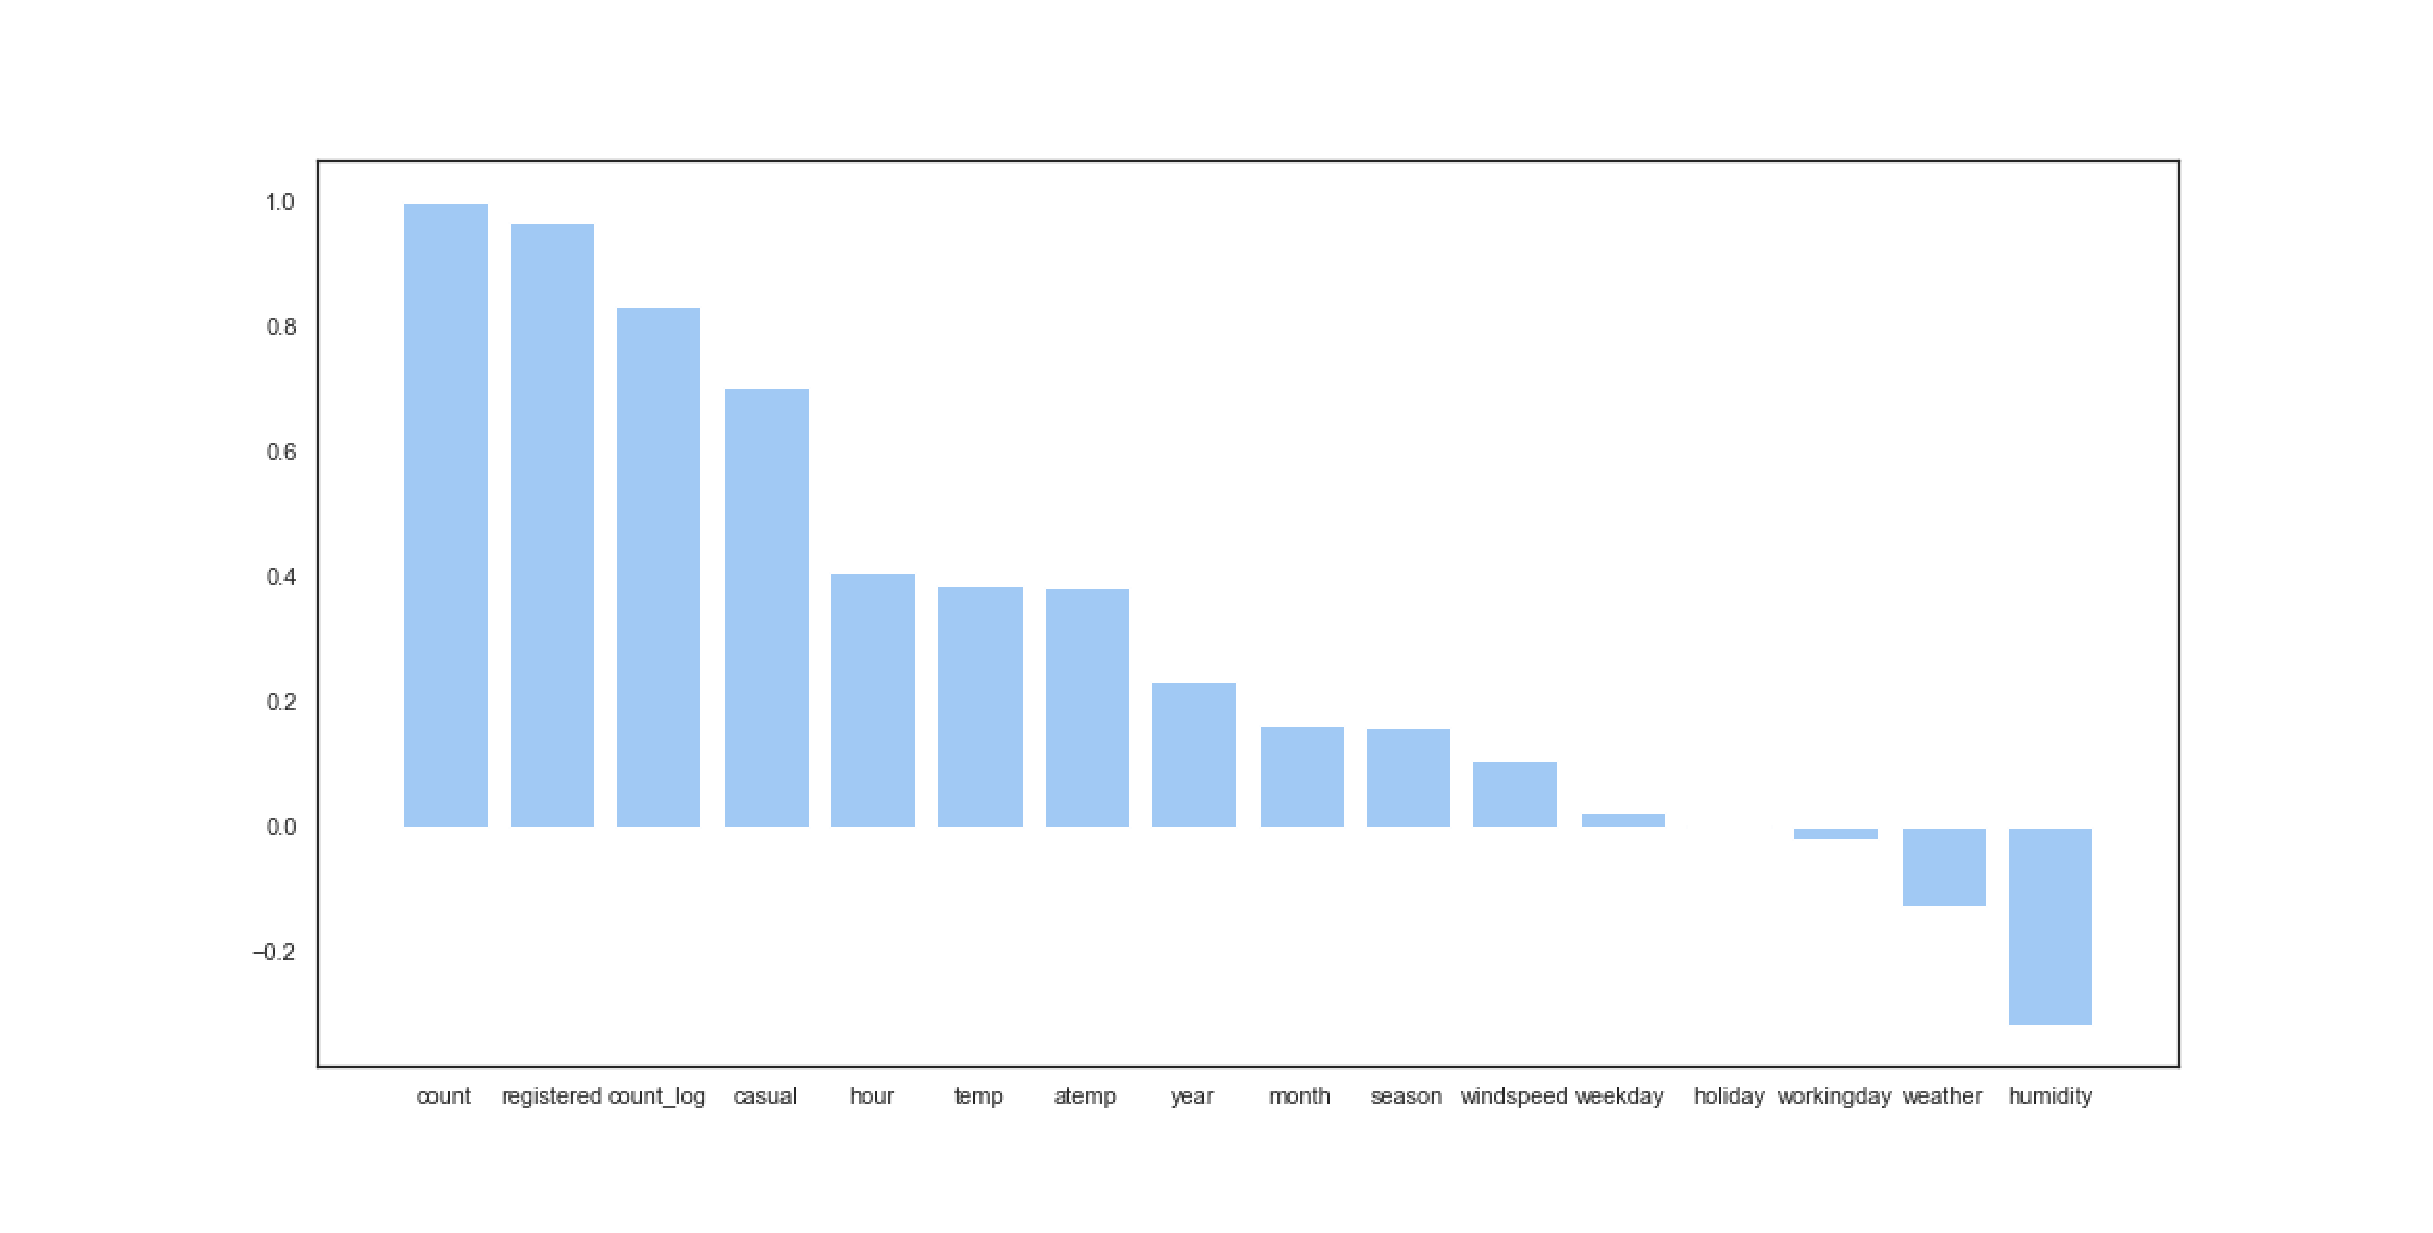
\includegraphics[width=0.8\textwidth]{figures//cor_rank.eps}\\
    \caption{Correlation rank} \label{framework}
  \end{figure}
  
  
  \end{slide}
%%
%%==========================================================================================
  
\section{Modelling and Forecasting}


%%==========================================================================================
%%
\begin{slide}{}
  
\begin{itemize}
\item
Select random forest model and cross validation using grid search
  
\end{itemize} 
\vspace{1.5cm}
\begin{tabular}{ c | c | c  }
\toprule
Result     &  The initial model    & After cross validation       \\
\midrule
Accuracy       &  0.9338   &  0.9249       \\
  
MSLE      &  0.0152   &  0.0159     \\
  
\bottomrule       
\end{tabular}



  
  
  
\end{slide}
%%
%%==========================================================================================
      


\section{Conclusion}


%%==========================================================================================
%%
\begin{slide}[toc=,bm=]{Evaluation}

\begin{center}
\begin{itemize}

\item
Cross-validation by grid search did not decrease the RMSE of the model and did not improve the accuracy of the model.
The effect did not come up to expectations.
The limitation of this study is that it does not consider whether there is overfitting of the model, and further experiments can be carried out in future studies.

\end{itemize}
\end{center}


\end{slide}
%%
%%==========================================================================================


%%==========================================================================================
%%
\begin{slide}{Synthetic Dataset}

\begin{itemize}
\item Synthetic Dataset and Ground Truth
\end{itemize}

\begin{table}
\setlength{\abovecaptionskip}{0pt}
\setlength{\belowcaptionskip}{10pt}
\centering
\caption{Synthetic Dataset and Ground Truth}

\begin{tabular}{p{2.8cm}p{0.9cm}p{0.9cm}p{0.9cm}p{0.9cm}p{0.9cm}p{0.9cm}p{0.9cm}p{0.9cm}}
\hline
  % after \\: \hline or \cline{col1-col2} \cline{col3-col4} ...
  Query group  & $\mathbf{F_1}$ & $\mathbf{F_2}$ & $F_3$ & $\mathbf{F_4}$ & $F_5$ & $F_6$ & $F_7$ & $F_8$\\
\hline
  $i_1$   & \bf{10} & \bf{8}  & 9  & \bf{7}  & 7 & 6 & 6  & 8\\
  $i_2$   & \bf{9}  & \bf{9}  & 7  & \bf{8}  & 9 & 9 & 8  & 9\\
  $i_3$   & \bf{8}  & \bf{10} & 8  & \bf{9}  & 6 & 8 & 7  & 8\\
  $i_4$   & \bf{8}  & \bf{8}  & 6  & \bf{7}  & 8 & 8 & 6  & 7\\
  $i_5$   & \bf{9}  & \bf{9}  & 9  & \bf{7}  & 7 & 7 & 8  & 8\\
  $i_6$   & \bf{8}  & \bf{10} & 8  & \bf{8}  & 6 & 6 & 8  & 7\\
  $i_7$   & \bf{9}  & \bf{9}  & 7  & \bf{9}  & 8 & 8 & 8  & 7\\
  $i_8$   & \bf{10} & \bf{9}  & 10 & \bf{7}  & 7 & 7 & 7  & 7\\
  $i_9$   & \bf{9}  & \bf{10} & 8  & \bf{8}  & 7 & 6 & 7  & 7\\
  $i_{10}$& \bf{9}  & \bf{9}  & 7  & \bf{7}  & 7 & 8 & 8  & 8\\
\hline
\end{tabular}
\end{table}

%%==========================================================================================
\begin{note}
Now,
I am gonna use a synthetic dataset to verify our method.

The dataset we used in our experiment contains $10$ groups,
each group consists of $10$ members,
and each member has $8$ features: $F_1$ to $F_8$.

Table $5$ shows the original data of one group,
and the bold features represent the ground truth,
The ground truth include trivial outlying feature \{$F_1$\},
and non-trivial outlying subspace \{$F_2$, $F_4$\}.
\end{note}
%%==========================================================================================

\end{slide}
%%
%%==========================================================================================


%%==========================================================================================
%%
\begin{slide}[toc=,bm=]{Synthetic Dataset Results}

\begin{table}[tb]
\setlength{\abovecaptionskip}{0pt}
\setlength{\belowcaptionskip}{10pt}
\centering
\caption{The experiment result on synthetic dataset}

\begin{tabular}{ c | c | c | c }
\toprule
  % after \\: \hline or \cline{col1-col2} \cline{col3-col4} ...
  Method     &  Truth Outlying Aspects    & Identified Aspects & Accuracy      \\
\midrule
  GOAM       &  $\{F_1\}$, $\{F_2F_4\}$   &  $\{F_1\}$, $\{F_2F_4\}$    & 100\%    \\

Arithmetic Mean based OAM &  $\{F_1\}$, $\{F_2F_4\}$   &  $\{F_4\}$, $\{F_2\}$    &  0\% \\

Median based OAM &  $\{F_1\}$, $\{F_2F_4\}$   &  $\{F_2\}$, $\{F_4\}$    &           0\% \\
\bottomrule
\end{tabular}
\end{table}

%%==========================================================================================
\begin{note}
From table $6$,
we can see that GOAM method can identify the trivial outlying features
and non-trivial outlying subspaces accurately and
it is obvious from the table that the accuracy of GOAM is the best,
which is 100\%.

This is because the outlying aspects mining method
can't obtain the features of a group and the scoring function
is based on point to point metric.
Therefore,
it is not suitable for group outlying aspects mining.
\end{note}
%%==========================================================================================

\end{slide}
%%
%%==========================================================================================


%%==========================================================================================
%%
\begin{slide}{NBA Dataset}
Data Collection
\begin{description}[type=1]
\item
Source\\
\qquad
\emph{Yahoo Sports} website (\url{http://sports.yahoo.com.cn/nba})

\item
Data

\begin{itemize}
 \item Extract NBA teams' data until March 30, 2018;
 \item 6 divisions;
 \item 12 features (eg: \emph{Point Scored}).
\end{itemize}
\end{description}

%%==========================================================================================
\begin{note}
Next,
I will illustrate it further by applying the GOAM algorithm to the NBA dataset.
The data was collected from Yahoo Sports website.

In our experiment,
a web crawler was deployed to extract data
for all NBA teams until March 30, 2018.
The data includes all teams from the six divisions,
and each player in the team has 12 features,
such as point scored, field goal\dots
\end{note}
%%==========================================================================================

\end{slide}
%%
%%==========================================================================================


%%==========================================================================================
%%
\begin{slide}[toc=,bm=]{NBA Dataset}
The detail features are as follows:

\begin{table}[tb]
\setlength{\abovecaptionskip}{0pt}
\setlength{\belowcaptionskip}{10pt}
\centering
\caption{Collected data of Brooklyn Nets Team}

\begin{tabular}{p{0.9cm}p{0.9cm}p{0.9cm}p{0.9cm}p{0.9cm}p{0.9cm}p{0.9cm}p{0.9cm}p{0.9cm}p{0.9cm}p{0.9cm}p{0.9cm}}
\hline
  Pts & FGA & FG\% & 3FA & 3PT\% & FTA & FT\% & Reb & Ass & To & Stl & Blk \\
\hline
  18   & 12    & 42 &2.00 & 50 & 7.00 & 100& 0& 4& 3& 0& 0 \\
  15.7 & 14.07 & 41 &5.45 & 32 & 3.05 & 75 & 3.98& 5.1& 2.98& 0.69& 0.36\\
  14.5 & 11.1  & 47 &0.82 & 26 & 4.87 & 78 & 6.82& 2.4& 1.74& 0.92& 0.66 \\
  13.5 & 10.8  & 42 &5.37 & 37 & 3.38 & 77 & 6.66& 2& 1.38& 0.83& 0.42 \\
  12.7 & 10.59 & 39 &5.36 & 33 & 3.37 & 82 & 3.24& 6.6& 1.56& 0.89& 0.31 \\
  12.6 & 10.93 & 40 &6.94 & 37 & 1.70 & 84 & 4.27& 1.5& 1.06& 0.61& 0.44 \\
  12.2 & 10.39 & 44 &3.42 & 35 & 2.70 & 72 & 3.79& 4.1& 2.15& 1.12& 0.32 \\
  10.6 & 7.85  & 49 &4.51 & 41 & 1.35 & 83 & 3.34& 1.6& 1.15 & 0.45& 0.24 \\
\hline
\end{tabular}
\end{table}

%%==========================================================================================
\begin{note}
Table $7$ shows part of the collected data.
From this table,
we can see that the feature values are continuous.
\end{note}
%%==========================================================================================

\end{slide}
%%
%%==========================================================================================


%%==========================================================================================
%%
\begin{slide}[toc=,bm=]{NBA Dataset}
\begin{itemize}
\item Data Preprocess
\end{itemize}

\begin{table}
\setlength{\abovecaptionskip}{0pt}
\setlength{\belowcaptionskip}{10pt}
\centering
\caption{The bins that used to discrete data of each feature}

\begin{tabular}{p{2.5cm}p{2cm}p{1.8cm}p{2cm}p{1.8cm}p{1.8cm}p{1.8cm}}
\hline
  Labels & Pts & FGA & FG\% & 3FA & 3PT\% & FTA  \\
\hline
  low &  [0,5]& [0,4] & [0,0.35] & [0,1.0] & [0,0.2] & [0,1.0] \\
  medium& (5,10]& (4,7] & (0.35,0.45] & (1.0,2.5]& (0.2,0.3] & (1.0,1.5] \\
  high &  (10,15] & (7,10] & (0.45,0.5] & (2.5,3.5]& (0.3,0.35]& (1.5,2.5] \\
  very high&(15,$+\infty$]& (10,$+\infty$] & (0.5,1] & (3.5,$+\infty$] & (0.35,1] & (2.5,$+\infty$] \\
\hline
 Labels & FT\% & Reb & Ass & To & Stl & Blk \\
\hline
  low   & [0,0.6] & [0,2.0] & [0,1.0] & [0,0.6] & [0,0.2] & [0,0.25] \\
  medium& (0.6,0.65]& (2,5] & (1,2] & (0.6,0.9] & (0.2,0.5] & (0.25,0.5] \\
  high  & (0.65,0.75] & (5,6] & (2,4] & (0.9,1.7] & (0.6,0.75] & (0.5,0.7] \\
  very high& (0.75,1] & (6,$+\infty$] & (4,$+\infty$] & (1.7,$+\infty$] & (0.75,$+\infty$] & (0.7,$+\infty$]\\
\hline
\end{tabular}
\end{table}

%%==========================================================================================
\begin{note}
For those features with continuous values,
we use the binning method to discretize them,
the results are shown in table $8$.

Once the data was prepared,
we added three teams in the eastern division
and three teams in the western division into the query group,
the other teams together belonged to the contrast groups.
\end{note}
%%==========================================================================================

\end{slide}
%%
%%==========================================================================================


%%==========================================================================================
%%
\begin{slide}[toc=,bm=]{NBA Dataset Results}

\begin{table}[htbp]
\setlength{\abovecaptionskip}{0pt}
\setlength{\belowcaptionskip}{10pt}
\centering
\caption{The identified outlying aspects of groups}

\begin{tabular}{ccc}
\hline
  Teams                   & Trivial Outlying Aspects  & NonTrivial Outlying Aspects    \\
\hline
  Cleveland Cavaliers     & \{3FA\}                   & \{FGA, FT\%\}, \{FGA, FG\%\} \\
  Orlando Magic           & \{Stl\}                   & None                         \\
  Milwaukee Bucks         & \{To\}, \{FTA\}           & \{FGA, FTA\}, \{3FA, FTA\}     \\
  Golden State Warriors   & \{FG\%\}                  & \{FT\%, Blk\}, \{FGA, 3PT\%, FTA\}\\
  Utah Jazz               & \{Blk\}                   & \{3FA, 3PT\%\}                    \\
  New Orleans Pelicans    & \{FT\%\}, \{FTA\}         & \{FTA, Stl\}, \{FTA, To\}          \\
\hline
\end{tabular}
\end{table}

%%==========================================================================================
\begin{note}
We can see the identified group outlying aspects of each team from table $9$.
It is very clear that the GOAM algorithm can identify the
Trivial Outlying Aspects and Non-Trivial Outlying Aspects of each team.
\end{note}
%%==========================================================================================

\end{slide}
%%
%%==========================================================================================


\section{Conclusion}

%%==========================================================================================
%%
\begin{slide}[toc=,bm=]{Conclusion}
\begin{itemize}
\item
\smallskip
Formalize the problem of \emph{Group Outlying Aspects Mining} by
extending outlying aspects mining;

\item
\smallskip
Propose a novel method \textcolor{orange}{GOAM algorithm} to solve the
\emph{Group Outlying Aspects Mining} problem;

\item
\smallskip
Utilize the pruning strategies to reduce time complexity.

\end{itemize}


\end{slide}
%%
%%==========================================================================================


%%==========================================================================================
%
\begin{slide}[toc=,bm=]{Questions?}
\begin{center}
\begin{figure}
    \animategraphics[autoplay, loop, height=0.4\textheight]{5}{figures//gif//question//q_}{1}{30}
\end{figure}
\end{center}
\end{slide}
%%
%%==========================================================================================


%%==========================================================================================
% TODO: Contact Page
\begin{wideslide}[toc=,bm=]{Contact Information}
\centering
\vspace{\stretch{1}}
\twocolumn[
lcolwidth=0.35\linewidth,
rcolwidth=0.65\linewidth
]
{
% \centerline{\includegraphics[scale=.2]{tulip-logo.eps}}
}
{
\vspace{\stretch{1}}
Associate Professor Gang Li\\
School of Information Technology\\
Deakin University, Australia
\begin{description}
 \item[\textcolor{orange}{\faEnvelope}] \href{mailto:gangli@tulip.org.au}
 {\textsc{\footnotesize{gangli@tulip.org.au}}}

 \item[\textcolor{orange}{\faHome}] \href{http://www.tulip.org.au}
 {\textsc{\footnotesize{Team for Universal Learning and Intelligent Processing}}}
\end{description}
}
\vspace{\stretch{1}}
\end{wideslide}

\end{document}

\endinput
